
%(BEGIN_QUESTION)
% Copyright 2007, Tony R. Kuphaldt, released under the Creative Commons Attribution License (v 1.0)
% This means you may do almost anything with this work of mine, so long as you give me proper credit

In both FOUNDATION Fieldbus H1 and Profibus PA, two fieldbus networks sharing the same physical layer (IEC 61158-2), {\it terminators} must be connected to both far ends of the cable.  These terminators consist of a 100 $\Omega$ resistor connected in series with a 1 $\mu$F capacitor.  Also, any DC power supply must be connected through a {\it power conditioner} in order for the network to function.  Both types of devices are shown in this diagram:

$$\includegraphics[width=15.5cm]{i02433x01.eps}$$

\vskip 10pt

Answer the following questions about the terminators and power conditioner:

\begin{itemize}
\item{} What is significant about the size of the resistor in each terminator (100 $\Omega$)?
\vskip 10pt
\item{} Why is each termination resistor connected in series with a 1 $\mu$F capacitor?  Why not terminate with just a plain 100 $\Omega$ resistor at each end of the network?
\vskip 10pt
\item{} What function does the power conditioner serve?  Specifically, what is the purpose of the 10 mH inductor connected in series?
\vskip 10pt
\item{} Is the resistor necessary in the power conditioner network?  Why or why not?
\vskip 10pt
\medskip

\vskip 20pt \vbox{\hrule \hbox{\strut \vrule{} {\bf Suggestions for Socratic discussion} \vrule} \hrule}

\begin{itemize}
\item{} If FOUNDATION Fieldbus H1 and Profibus PA share the same physical layer, does that mean the two types of instruments will work interchangeably on the two types of networks?  Will a FF instrument be damaged by plugging it into a PA network, or visa versa?  Why or why not? 
\item{} In order for a HART instrument to work, there must be at least 250 ohms of loop resistance present.  Explain why this is, and also identify the equivalent feature within a FOUNDATION Fieldbus H1 network.
\item{} Explain why the termination resistors used in digital networks such as RS-485 and Ethernet do {\it not} require series capacitors like the terminators in FF networks do.
\item{} Can you use a digital multimeter (DMM) to detect the presence of FOUNDATION Fieldbus data signals?  Why or why not?
\end{itemize}

\underbar{file i02433}
%(END_QUESTION)





%(BEGIN_ANSWER)

\noindent
{\bf Partial answer:}

\begin{itemize}
\item{} What is significant about the size of the resistor in each terminator (100 $\Omega$)?
\vskip 10pt
\item{} Why is each termination resistor connected in series with a 1 $\mu$F capacitor?  Why not terminate with just a plain 100 $\Omega$ resistor at each end of the network? {\it Capacitive coupling is necessary because the network also carries DC power.}
\vskip 10pt
\item{} What function does the power conditioner serve?  Specifically, what is the purpose of the 10 mH inductor connected in series?  {\it The power conditioner blocks the fieldbus communication signals from being shorted out by the DC voltage source.}
\vskip 10pt
\item{} Is the resistor necessary in the power conditioner network?  Why or why not? {\it It is there for current limiting and also anti-resonance.}
\vskip 10pt
\medskip

%(END_ANSWER)





%(BEGIN_NOTES)

\begin{itemize}
\item{} What is significant about the size of the resistor in each terminator (100 $\Omega$)?  {\it It matches the characteristic impedance of the cable (Types A and B, at least), which is necessary to avoid reflected signals.}
\vskip 10pt
\item{} Why is each termination resistor connected in series with a 1 $\mu$F capacitor?  Why not terminate with just a plain 100 $\Omega$ resistor at each end of the network? {\it Capacitive coupling is necessary because the network also carries DC power.  A plain resistor would act as a relatively heavy load on the power source, drawing 240 mA of current and dissipating over 5 watts of power each!}
\vskip 10pt
\item{} What function does the power conditioner serve?  Specifically, what is the purpose of the 10 mH inductor connected in series?  {\it The power conditioner blocks the fieldbus communication signals from being shorted out by the DC voltage source, much like the mandatory loop resistance of a HART hybrid analog/digital circuit.  The series inductor presents a substantial impedance to the network signals.}
\vskip 10pt
\item{} Is the resistor necessary in the power conditioner network?  Why or why not? {\it It is there for current limiting and also anti-resonance (to dampen oscillations that might otherwise result from interaction between the inductor and network capacitance).}
\vskip 10pt
\medskip

\vskip 10pt

Note: the DC power supply needs to be floating (ungrounded), or else the fieldbus power conditioner needs to provide electrical isolation from ground!

\vskip 20pt \vbox{\hrule \hbox{\strut \vrule{} {\bf Virtual Troubleshooting} \vrule} \hrule}

This question is a good candidate for a ``Virtual Troubleshooting'' exercise.  Presenting the diagram to students, you first imagine in your own mind a particular fault in the system.  Then, you present one or more symptoms of that fault (something noticeable by an operator or other user of the system).  Students then propose various diagnostic tests to perform on this system to identify the nature and location of the fault, as though they were technicians trying to troubleshoot the problem.  Your job is to tell them what the result(s) would be for each of the proposed diagnostic tests, documenting those results where all the students can see.

During and after the exercise, it is good to ask students follow-up questions such as:

\begin{itemize}
\item{} What does the result of the last diagnostic test tell you about the fault?
\item{} Suppose the results of the last diagnostic test were different.  What then would that result tell you about the fault?
\item{} Is the last diagnostic test the best one we could do?
\item{} What would be the ideal order of tests, to diagnose the problem in as few steps as possible?
\end{itemize}

%INDEX% Fieldbus, FOUNDATION (H1): power conditioners
%INDEX% Fieldbus, Profibus PA: power conditioners
%INDEX% Fieldbus, FOUNDATION (H1): terminators
%INDEX% Fieldbus, Profibus PA: terminators

%(END_NOTES)


